\section{Vehicle Sizing} \label{section:sizing}
\subsection{Introduction}
In order to verify that our vehicle is able to satisfy the mission requirements it is vital to have an understanding of what a proposed vehicle would look like in terms of its design aspects. Factors that include propulsive, structural, aerodynamic, thermal, and many others must be considered in order to properly assess if a contending vehicle design is viable in terms of matching requirements for the mission's success.

A large trade study was conducted in order to find a vehicle design that meets the individual requirements of each subteam. Since it was determined that the propulsion system of the launch vehicle has the most direct influence in a given design's ability to achieve the desired mission objectives, the figure of merit analysis started with the propulsion design.

The sizing process began at the highest level possible, evaluating the entire vehicle system. Our scope was then increasingly refined and candidate designs were filtered until only handful of viable point designs remained, all of which satisfactorily met our mission requirements.

This process first used a Pareto analysis to generate a large dataset of possible candidate designs. Then a 1-degree of freedom (1DOF) mathematical model was used to determine the propulsion requirements for each point design as well as forecast a projected time history of resulting flight to space. The propulsion analysis calculated metrics like propellant mass required and motor burn times, and the time history tracked flight parameters such as dynamic pressure experienced and delta-V split between the two stages. This data was then sifted through by the aerostructures team that looked at factors such as chamber pressure and temperature history, motor dimensions, inert mass, among others, to determine if designs were realistic candidates for further analysis. A point design was thrown out if the inert mass required to match the specified safety factors for structural stability was deemed to not be achievable. In the final step of this process, a comprehensive 6-degree of freedom (6DOF) mathematical model study was conducted that served two purposes: give a refined trajectory of the vehicle’s mission, and verify that the outputs from the 1-dimensional model were reasonable, which gave a sanity check to the entire process. Ultimately the 6DOF gave a finishing polish on the process, giving the team confidence that the selected point designs had a high probability of completing the mission requirements successfully.

The validity of this process --- the down-selecting of viable vehicle designs that satisfy all the mission requirements --- is yet to be shown experimentally. However, we believe our outlined methodology to be sound on a conceptual level go on to document our assumptions, procedures and decisions in the following sections of this report.


\subsection{Figure of Merit and Pareto Analysis}
The Pareto analysis, a formal technique which may be useful where many possible courses of action are competing for attention, was paired with a figure of merit analysis that allowed both methods to complement each other with the desired goal of finding how the multitude of input parameters affected the performance of a point design, and then show how the many point designs compared against each other. The figure of merit analysis generated a set of point designs for a possible launch vehicle with the parameters that were simulated summarized in \Cref{table:pareto-parameters}, with every combination of parameters being a point design tested.

\begin{table}
    \centering
    \begin{tabular}{|l|c|c|}
        \hline
        \textbf{Parameter} & \textbf{Initial Run} & \textbf{Final Run} \\ \hline
        First Stage Diameter (in) & 3.75, 4.0, 4.25, 4.5, 5.0 & 5.0, 5.25, 5.5 \\ \hline
        Second Stage Diameter (in) & 3.0, 3.5, 4.0, 4.5 & 4.0, 4.25, 4.5, 4.75 \\ \hline
        Payload Mass (kg) & 1, 3, 4, 5, 10 & 0.5 \\ \hline
        Desired Apogee Altitude (km) & 100, 125, 150, 200, 250, 300, 400 & 100, 125, 150 \\ \hline
        First Stage \(\Delta V\) Split & 35\%, 40\%, 45\%, 50\%, 55\%, 65\% & 35\%, 42.5\% \\ \hline
        Propellant Mass Fraction (\(\lambda_p\)) & \(\lambda_{p,1}\) = 0.85 \quad \(\lambda_{p,2}\) = 0.785 & \(\lambda_{p,1} = 0.7 \quad \lambda_{p,2} = 0.6\) \\ \hline
        \(I_{sp}\) Efficiency (\(\eta_{isp}\)) & 0.925 & 0.9 \\ \hline
        Total Point Designs Tested & 4200 & 72 \\ \hline
    \end{tabular}
    \caption{Summary of Pareto analysis vehicle parameters}
    \label{table:pareto-parameters}
\end{table}

Each point design was evaluated using both the 1DOF model and the genetic algorithm, with the 1DOF model being the main computational engine in the sizing process. The genetic algorithm iterated on chamber pressure profiles for the first and second stage motors in order to maximize the following characteristic evaluation function.

\begin{multline*}
    CEF = W_1 \left(1 - \frac{t_{ref}}{t_{b1} + t_{b2}}\right) + W_2 \left(\frac{m_{pl}}{m_{pl,ref}}\right) + W_3 \left(\frac{h}{h_{ref}} - 1\right) \\ 
    + W_4 \left(1 - \frac{m_{p,ref} - m_p}{m_{p,ref}}\right) + W_5 \left(1 - \frac{Q_{max,ref}}{Q_{max}}\right) + W_6 \left(1 - \left[\frac{L/D_{ref} - L/D}{L/D_{ref}}\right]^2\right)
\end{multline*}

\begin{table}
    \centering
    \begin{tabular}{cccccc}
        \(W_1\) & \(W_2\) & \(W_3\) & \(W_4\) & \(W_5\) & \(W_6\) \\ \hline
        -0.4 & 0.05 & 0.35 & -0.4 & -0.2 & 0.6
    \end{tabular}
    \vspace{0.3cm} \\
    \begin{tabular}{cccccc}
        \(t_{ref}\) & \(m_{pl,ref}\) & \(h_{ref}\) & \(m_{p,ref}\) & \(Q_{max}\) & \(L/D_{ref}\) \\ \hline
        10 sec & 5 kg & 103.57 km & 119.522 kg & 200 kPa & 19.5
    \end{tabular}
    \caption{Characteristic evaluation function weights and reference values}
    \label{table:CEF-weights-ref}
\end{table}

This characteristic evaluation function was the backbone to the Pareto analysis, which included six metrics that were chosen to best represent the performance of a potential design. The metrics chosen were: burnout times for the first and second stage (\(t_b\)), payload mass (\(m_{pl}\)), altitude at apogee (\(h\)), mass of propellant for first and second stage (\(m_p\)), maximum dynamic pressure experienced (\(Q_{max}\)), and aspect ratio for the entire vehicle (\(L/D\)). Reference values were utilized in the characteristic evaluation function in order to normalize the data as best as possible, with the values used being summarized in \Cref{table:CEF-weights-ref}. The weights chosen by our team as the values of \(W\) are designed to put emphasis on parameters deemed more impactful to the mission, and factors that have an unfavorable impact on the design have negative sign. In all, the characteristic evaluation function (CEF) is bound between -1 and 1, with a design performing the best with a score of 1. The overall distribution for point designs score of the CEF was modeled to be approximately normal. The reference values are modeled after Traveler IV, with the exception of \(t_{ref}\), \(m_{pl,ref}\), and \(Q_{max}\), which were all chosen using a point estimation for the population mean of the point designs tested in the set. Parameters such as desired altitude, payload mass, and to an extent aspect ratio are all direct input parameters to the system, whereas the rest of the values are outputs from the 1DOF model.

A plot for an example batch of point designs that have been normalized within the set are shown in \Cref{figure:pareto-points}, where the ``value'' is defined as the factors in the CEF that are positive, and the ``cost'' are the factors that are negative. The point designs that are colored in red are chosen as favorable designs since they have the best balance between the costs and value, whereas the blue labeled points have corresponding designs that may perform at the same value but with minimal cost. This method of screening was used for the initial selection process for viable point designs. This region of red dots is known as the Pareto Frontier, and the slope of the frontier shows a direct visual trade off of certain parameters of a point design to the overall performance.

\begin{figure}
    \centering
    \begin{tikzpicture}
        \begin{axis}[
            width=12cm,
            height=10cm,
            xlabel={Cost},
            ylabel={Value},
            xmin=0.7, xmax=1.0,
            ymin=0.4, ymax=1.0,
            xtick={0.7, 0.75, 0.8, 0.85, 0.9, 0.95, 1.0},
            xticklabels={0.7, 0.75, 0.8, 0.85, 0.9, 0.95, 1.0},
            ytick={0.4, 0.5, 0.6, 0.7, 0.8, 0.9, 1.0},
            yticklabels={0.4, 0.5, 0.6, 0.7, 0.8, 0.9, 1.0},
            xmajorgrids=true,
            ymajorgrids=true,
            ticklabel style = {font=\small},
        ]
            \addplot[
                only marks,
                red,
                mark=o,
                mark size=3pt,
            ]
            table{data/pareto-red.csv};
            \addplot[
                only marks,
                blue,
                mark=o,
                mark size=3pt,
            ]
            table{data/pareto-blue.csv};
        \end{axis}
    \end{tikzpicture}
    \caption{Pareto analysis results scatter plot}
    \label{figure:pareto-points}
\end{figure}


The genetic algorithm used converged on a point design when the characteristic evaluation function was maximized for a given chamber pressure profile. In order to best prevent the program from settling on a local maximum, a few measures were implemented to find the solution which converged with the highest value which was the best approximation of a global maximum. The first generation that was run through the 1DOF model used a seed profile with a total of 7 ``offspring'' profiles, which were altered versions of the seed profile. Of the offspring, 4 were more conservative variations that were intended to refine the parent generation with minor adjustments, whose purpose was to converge on a local maximum of the characteristic evaluation function. The 3 other offspring profiles had much larger changes from the parent generation which are designed to bump the convergence from one local maximum to another. After the 8 profiles converged, the overall best score from the characteristic function was found, which then was chosen as the next parent seed for the following generation. This process was repeated for the designated amount of generations by the user. A visual example of this process is shown below in \Cref{figure:genetic-chamber-pressure}, where an example is shown after all schemes have been tested, and the darkened profile is selected as the parent profile for the next generation since it has the highest characteristic evaluation function score. The entire selection process is simplified in the flowchart in \Cref{figure:genetic-flowchart}.

\begin{figure}
    \centering
    \includegraphics[width=0.7\linewidth]{images/genetic-chamber-pressure}
    \caption{Example genetic algorithm run}
    \label{figure:genetic-chamber-pressure}
\end{figure}


\begin{figure}
    \centering
    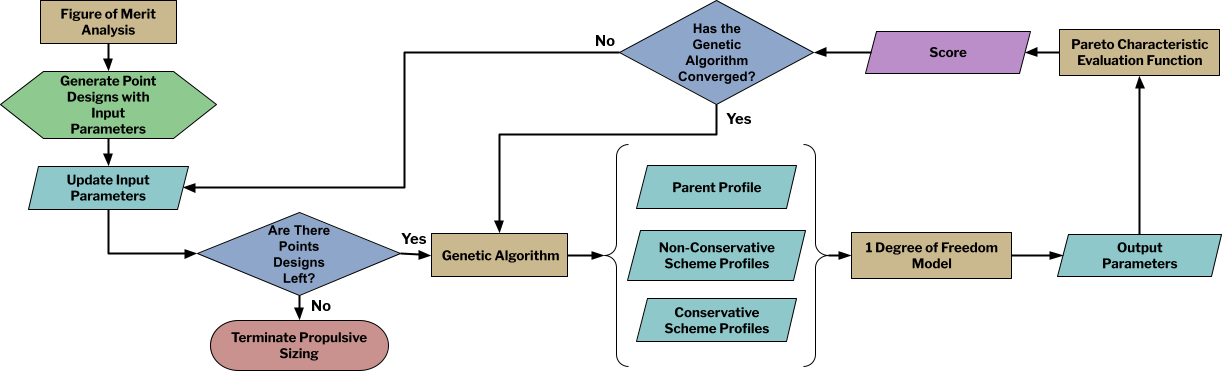
\includegraphics[width=\linewidth]{images/genetic-flowchart}
    \caption{Genetic algorithm selection process flowchart}
    \label{figure:genetic-flowchart}
\end{figure}


\subsection{One Degree of Freedom Analysis}
The 1DOF utilized in this process started by initializing a few key parameters that were held constant in each subsequent point design, which included: propellant characteristics and composition, nozzle characteristics with expansion ratio, empirical estimations for propellant mass fractions, and empirical estimation for \(I_{sp}\) efficiency.

These aspects were held to be constant with one notable exception, the propellant mass fraction estimate. Using historical data provided in Figure 3.4 of ``Rocket Propulsion'' \cite{heister-rocket-propulsion} a rough approximation was made for the propellant mass fraction, which relates the total mass of the motor to the mass of propellant. It was found later from the structures sub team, that these empirical estimations were giving values for acceptable inert masses to be less than what could be reasonably done, therefore these values had to be adjusted in order to give more inert mass to each stage so an appropriate aerostructure could be designed while fitting the designated inert mass budget. The propellant mass fraction was different for both the first and second stage, with the second stage having more inert mass accounted for, and likewise a lower inert mass fraction, due to an interstage and other factors due to the two stage nature of the vehicle.

The propellant characteristics were not adjusted due to the limitation from faculty advisors to not develop our own proprietary propellant, which would allow for individual tailoring of different traits. This limited our total selection of propellants severely, and ultimately a propellant (TS - 78) derived from published literature from NATO was  selected due to its high performance and relatively safe manufacturability. In further testing for the mission this input parameter of propellant performance will have the most direct impact on this model’s results. Currently, the propellant is modeled using NASA CEA to give motor characteristics such as: exhaust velocity, chamber temperature, motor characteristic velocity, motor ISP, and exhaust static pressure. Further tests will give improved representations of these factors.

The nozzle was held constant since it added a few extra variables to the selection process, namely throat area, exit area, and therefore expansion ratio. It was decided that these factors could be adjusted after the selection process was done if need be.

In order to properly have a solution from the 1DOF, iteration was relied on heavily to fully define the variables in the system. The main variable that was iterated upon was the mission’s total change in velocity (\(\Delta V\)), which trickled down to a few other variables. If a value for total \(\Delta V\) was estimated, then using the ideal rocket equation with the propellant mass fractions and the stage specific impulse, a value for the vehicle's mass could be found broken up between first and second stage for its inert and propellant mass. Then, once propellant mass is found for each stage, burn time per motor can be iterated upon using the mass flow rate history of each stage (derived from the chamber pressure profile, throat area, and characteristic velocity) until the total mass accumulated is equivalent to the propellant mass found with the ideal rocket equation. Following this, an atmospheric model was utilized to find aerodynamic forces on the vehicle. The flight of the vehicle was modeled using a time stepping force balance that accounted for the mass exhausted from the motor and the thrust of the motor, drag, and gravity in order to find the acceleration at a designated time. Velocity was found from the integration of acceleration, and so forth for altitude. It is key to note that all thrust was modeled to be purely axial, all aerodynamic forces were axial, and likewise with body forces from gravity. After a motor had burnt out, a coasting period was modeled, if required by the input parameters of the mission, by the same procedure just without thrust of the motor. Once separation occurred, the inert mass of the first stage was subtracted from the vehicles total mass, and the second stage followed the same procedure to find acceleration on the vehicle. This process resulted in the time history data for vehicle mass, dynamic pressure, net force, acceleration, velocity, altitude, atmospheric conditions, Mach, along with others derived from these. It is important to note that the coefficient of drag used in this model was variable and had critical Mach numbers of 0.7 and 1.3, which affected the vehicle most as it was going through Mach 1. After all of these calculations took place, the final altitude was compared to the input parameter for the desired altitude, and if the margin of error was not met, the process would be repeated with an updated delta V for the mission. Therefore this method can be thought of as a modified ideal rocket solution, since at its core it uses the ideal rocket equation to find the mass of the vehicle, but it iterates on this value to find a solution that incorporates forces other than the vehicle's thrust.


\subsection{Mass Estimation and Sizing System}
Once the propulsion team generated point designs using ranges of parameters, it was decided that further steps were necessary to visualize and analyze the selected designs, as well as generate the inputs needed to evaluate the designs using the 6 degree of freedom (6DOF) model, which will be discussed in detail in \Cref{section:6dof}. The goal of this script is to determine whether point designs can fit the propulsion analysis' inert mass requirement, while doing preliminary structural analysis to ensure these materials and geometries pass minimum safety factor requirements.


\subsubsection{General Operation and Information}
The program takes inputs from the Pareto analysis, as well as from preliminary mass and location estimates for the vehicle subsystems. Using the inputs gathered from these sources, the program then does the basic geometric layout of the rocket, generating lengths, wall thicknesses, and a design that can then be visualized with the help of tools such as OpenRocket and CAD software. The program also calculates key physical characteristics of the rocket, the center of mass and mass moment of inertia over the duration of the flight.

In order to simplify analysis, some assumptions about the rocket were made, which are covered in \Cref{table:mass-script-assumptions}. The design generated contains the position and mass of all aerostructures and internal components from both stages. These include the nosecone, the sustainer airframe, the sustainer fins, the interstage, the booster airframe, and the booster fins. Internal components include the motor, the forward closure, the nozzle, the recovery subsystem, the despin subsystem, and the avionics subsystem.

\begin{table}
    \centering
    \begin{tabular}{ | >{\raggedright}p{0.38\textwidth} | p{0.58\textwidth} | } \hline  %TODO: raggedright both cols
        \textbf{Current Assumption} & \textbf{Justification} \\ \hline
        All point designs are sub-minimum diameter & The sub-minimum design, when compared to their minimum, and other counterparts for such high powered applications, offered more benefits in mass and space saving. \\ \hline
        All point designs use metallic airframes & Sub-minimum diameter rockets require their airframes to be pressure vessels, and the team does not have the capability to make composite overwrapped pressure vessels in-house. \\ \hline
        All point designs use four fins for each stage & This assumption was made in order to perform first-order analysis; in the future, fin characteristics will be optimized by the 6DOF and prior art. \\ \hline
        All point designs have a 5:1 Von Karman nosecone & Based on prior art; for other high powered rockets the 5:1 Von Karman design was commonly used. \\ \hline
        Point designs do not have igniters, RF-transparent sections, nozzles, fasteners, or couplers & These components are a part of the detailed design, as such to reduce complexity, they were left out of the analysis. \\ \hline
        All point designs' internal rocket components' dimensions and masses are static & These components are a part of the detailed design, as such to reduce complexity, they were left static in this analysis \\ \hline
        All point designs' internal components are modeled as cylinders & In order to simplify for the first order analysis, as well as generalize for the wide range of point designs generated, the internal subteams provided us with simplified representations of their sub-systems \\ \hline
    \end{tabular}
    \caption{Mass estimation and sizing assumptions}
    \label{table:mass-script-assumptions}
\end{table}

The program also performs primary column buckling and local column buckling analysis on the sustainer airframe. This is done assuming the airframe is a fixed-free column; however this will change once the detailed design of the rocket is done. Currently this check is simply a ``sanity check'' so to speak, just as a qualifier for further analysis on each point design.


\subsubsection{Analysis}

The Pareto analysis provided the diameters of both stages, the maximum expected operating pressure (MEOP) of both motors, the mass of the motors as a function of time, the maximum drag force, and the maximum acceleration of the rocket. Additional inputs were also given in the form of material properties, and geometric properties.

The majority of the analysis was performed on the airframes, as the dimensions and stability of the airframe drive the viability of the point design.

Starting with the airframes, wall thickness of each stage was calculated using the MEOP of both motors and the thin wall hoop stress formula. The length of the motor is calculated using the propellant mass, the propellant density, and the internal diameter of the airframes. The forward closure was modeled as a uniformly loaded circular disk with clamped edges, and thickness was backsolved from the corresponding formula. The length was calculated by simply adding the length of the motor, the internals, and the bulkheads together, with some amount of room for error. The mass of the airframe and the bulkheads was calculated by calculating the volume of each and multiplying by material density. The script has three types of column buckling included, with two relevant criteria per airframe. The first, the primary buckling instability can be modeled by either the Euler or Johnson buckling formulas. The script chooses one over the other based on the slenderness ratio of the airframe and calculates the associated buckling stress. The third form of analysis is local buckling. The formula was obtained from NASA’s SP 8007 manual \cite{nasa-sp8007}, and used to calculate the critical local buckling stress.

To estimate inert masses, a simple method was used. For aerostructures, we calculated the volume of each component and multiplied by material density. For the internal components, the internal subteams were consulted on generalized masses and dimensions for each sub system that could be applied to all point designs. The motor mass was given by the Pareto analysis outputs, and is represented as a function of mass over the time duration of the flight.

The script calculates the center of mass of the rocket as a function of time, based on the motor mass time history, and was verified at the beginning and end of motor burns using OpenRocket. It also calculates the moment of inertia of the vehicle in its three principal dimensions. This was verified using SolidWorks models of point designs.


\subsubsection{Results}
After the Pareto analysis determined a significant number of viable point designs, the structures script was used to further narrow down this number. Most point designs were discarded because they could not meet inert mass requirements, while others were deemed to have motors that would be beyond our team’s manufacturing capabilities. We used the 1DOF model to simulate all designs with an altitude ceiling of 150 km, however, the 6DOF model was not ready to validate or update this parameter. 6DOF validation of these point designs will likely bring down their flight ceiling significantly, and the extra altitude provides a mass budget excess that can be used in detailed design.

The materials and geometries used in the conceptual designs are primarily outlined in \Cref{section:structures}, but the materials (aluminum, titanium, steel) were chosen for their availability, manufacturability, thermal resistance, and strength, while geometries were chosen based on prior art and manufacturability. Following the structures analysis and its simplifying assumptions, the design space determined viable point designs were found within the bounds in \Cref{table:sizing-bounds}.

\begin{table}
    \centering
    \begin{tabular}{l|c|c}
        \textbf{Variable} & \textbf{Minimum Value} & \textbf{Maximum Value} \\ \hline
        Inert Mass & 14.39 kg & 18.39 kg \\
        Propellant Mass & 28.73 kg & 34.58 kg \\
        Stage 1 Diameter & 4.5 in & 5.5 in \\
        Stage 2 Diameter & 4.0 in & 4.75 in \\
        Burn Times & 6.1 sec & 9.1 sec \\
        Inert Mass Fraction & 63\% & 67\% \\
        Delta V Split & 35\% & 42.5\% \\
        Max. Mach Number & 6.5 & 8.0
    \end{tabular}
    \caption{Design space determined by the structures sizing process}
    \label{table:sizing-bounds}
\end{table}


As stated in \hyperlink{SR.4}{SR.4}, the team wishes to have an expendable first stage. This appears viable examining prior spaceshot launches, but confirmation is needed. Sizing has established that viable point designs exist with first stages that are not recoverable, such as the 4.5 to 4 inch rocket in \Cref{figure:smaller-point}. Additionally, viable point designs exist for fully recoverable rockets, such as the 5.5 to 4.75 inch rocket in \Cref{figure:larger-point}.

\begin{figure}
    \centering
    \includegraphics[width=\textwidth]{images/4-4.5-sizing}
    \caption{The 4''-4.5'' design, shown in its expendable configuration}
    \label{figure:smaller-point}
\end{figure}

\begin{figure}
    \centering
    \includegraphics[width=\textwidth]{images/4.75-5.5-sizing}
    \caption{The 4.75''-5.5'' design, which can reasonably be flown with either a recoverable or expendable first stage}
    \label{figure:larger-point}
\end{figure}

Throughout the rest of this report the work required to arrive at this design space will be presented. All of the work requiring dimensions and masses was done with the 4 to 4.5 inch expendable rocket, as this design represents the team’s Minimum Viable Product (MVP). Once the 6DOF can evaluate the design space, then additional analysis will be performed to ensure that the assumptions and Pareto analysis still hold true.



\subsection{Trajectory Analysis Model and Statistical Methods (6DOF)} \label{section:6dof}

Once a thorough primary design analysis is complete, the rocket must be simulated.  To conduct more thorough analysis of the point designs identified by the initial sizing process, HA developed a six degree of freedom (6DOF) model, to simulate the flight of a design to a much higher level of accuracy. We decided to progress directly from a 1DOF to a 6DOF, since building an intermediate 3DOF would not have been easily adaptable into a 6DOF. This model will be refined as the program develops, and will eventually be used to determine the confidence interval on the rocket’s apogee, and the landing ellipse where each stage will touch down.

The 6DOF model we developed runs in MATLAB Simulink. All the aerodynamic data is generated by a 1997 version of Missile DATCOM. While the most updated versions of this software are export controlled, the 1997 version is approved for public release and uncontrolled. Aerodynamic tables are generated in DATCOM; a table corresponds to a single rocket geometry over a range of altitudes, Mach numbers, combined sideslip and  angle of attack, and roll angles. The 6DOF numerically integrates the dynamic equations of motion corresponding to both position and orientation.

The 6DOF models the rocket’s motion in three spatial dimensions and their respective rotational modes as a result of in-flight forces, namely, thrust, gravity, and aerodynamics. A full attitude representation is given with respect to a geodetic frame, which has its third basis vector pointed at the center of the Earth. It also models motion relative to a rotating Earth and the included effects. The 6DOF requires an initialization script consisting of initial conditions for all relevant differential equations, atmospheric effects, Earth effects, an aerodynamic reference table for all stability derivatives, and design-specific variables: these are mass histories, MOI histories, center of mass, and thrust curves for both stages.. Once the simulation has run, a post-processing script provides trajectory visualization. Additionally, the simulation has the capability for dispersion analysis (currently only for apogee dispersion with a confidence ellipsoid) but only if the proper covariance is available. The simulation primarily uses discrete integration.


\subsubsection{Strengths and Shortcomings}
The 6DOF as it exists currently is not in its final state; there are a number of refinements planned for future semesters. However, analyses done for this report still contain the somewhat simplified assumptions of the current 6DOF. In \Cref{table:6dof-assumptions}, the assumptions made by the current model are enumerated, along with the planned improvements, when relevant.

\begin{table}
    \centering
    \begin{tabularx}{0.95\textwidth}{|>{\raggedright\arraybackslash}p{0.35\textwidth}|>{\raggedright\arraybackslash}X|}
        \hline
        \textbf{Current Assumption} & \textbf{Explanation / Planned Improvement} \\ \hline
        Wind/discrete gusts not considered & We plan to use the wind/gust model built into Simulink \\ \hline
        The rocket geometry is currently axisymmetric & This simplifies the dynamic model and the workload for the structures team without any significant loss in fidelity \\ \hline
        The simulation stops at apogee & In the near future, we will model the parachute deployments and descents, including drift \\ \hline
        Staging is perfect & We may add randomly-varying moments and forces on the stages at separation \\ \hline
        Staging is instantaneous & DATCOM cannot simulate the aerodynamic properties of two bodies in proximity; within the 6DOF, we will continue to neglect the dynamics of staging and focus only on the body of primary analysis \\ \hline
        Spin stabilization and de-spin are not modeled & As the stability analyses develop, this capability will be added to the 6DOF \\ \hline
        Thrust curve does not vary (constant thrust during burn) & As the design of the motors develops, realistic error will be injected into the thrust tables to model real variance of solid motors \\ \hline
        Thrust is perfectly aligned through the body primary axis & We will add random variability in the direction of the thrust, to simulate minor misalignments of the motor in the airframe \\ \hline
        Simulation starts right off the rail (neglects complex dynamics on the rail) & Since the dynamics of the rocket on the rail are very important to the overall trajectory, we are working to develop and integrate a rail model into the 6DOF with friction and added noise \\ \hline
    \end{tabularx}
    \caption{Summary of current 6DOF assumptions}
    \label{table:6dof-assumptions}
\end{table}

A strength of our model is its flexibility in rocket geometry; we can completely specify the geometry, and must only generate a new aerodynamic table with Missile DATCOM. We can also track any variable or any group of variables against each other using the MATLAB Simulink data inspector and scopes for real-time analysis. While this will be very useful as the detailed design of the vehicle converges, the breadth of the design space in these initial stages can be daunting. Since a single aerodynamic table generation takes upwards of a half hour, we are reluctant to generate many tables; instead we are working on how to appropriately and reasonably interpolate inside of the tables for reasonably small design changes. This process is not trivial and will take time and input from others to achieve.

\subsubsection{Stability}
An important task for the 6DOF is to ensure the vehicle is suitably stable at all phases of the flight. Many rockets with similar missions spin-stabilize; this is a possibility we are still evaluating. In the future, we will simulate flights with canted fins, for example, and compare the stability to flights with un-canted fins. It is likely that the vehicle will spin some amount even without canted fins, due to manufacturing tolerances, and this is also something that will need to be characterized.

We plan to perform basic transient stability analyses on the aerodynamic coefficients throughout the flight.  As some of the coefficients behave like damping terms in a classical mass-spring-damper system, we observe decaying sinusoidal motion in the stability derivatives with respect to time. Analyzing parameters like rise time, peak time, steady state, overshoot, and other factors can allow us to assess the raw stability of the system in the context of converging to a steady state, such as a small (preferably near-zero) angle of attack and sideslip angle, steady rolling motion, and small pitching/yawing oscillations. Beyond this, our team is currently working on a rigorous stability analysis methodology that will allow us to analyze a design or compare it to an ideal case. Additionally, the transonic flight regime will be scrutinized to a high degree as it is a key area of interest regarding flight stability. From there, specific CFD cases can be defined and investigated.


\subsubsection{Statistical Methods}
For higher-fidelity results, a single simulation per configuration will be insufficient. To properly characterize the influences of the many unknown components of the vehicle’s flight, we will need to perform hundreds or thousands of flights with the same configuration, only varying the noise and sources of error. We expect the most significant sources of noise in a real flight to be

\begin{itemize}
    \item Wind / turbulence
    \item The launch rail, and the forces it puts on the vehicle
    \item Manufacturing tolerances in the vehicle, especially the fins
    \item Variance in the motors, in terms of total impulse, the particular thrust curve, and the axis of thrust
    \item Large and quick disturbances in the turbulence of transonic flight
    \item Staging interactions
\end{itemize}

Moving forward, the primary metrics we will characterize probabilistically will be the apogee, and the landing locations for each stage. With the planned improvements in \Cref{table:6dof-assumptions} implemented, we will be able to run Monte-Carlo type analyses to determine confidence intervals on these two metrics. Currently, a chi-squared analysis is in place based on very basic covariance data to determine a ``confidence ellipsoid,'' wherein the rocket is expected to be at apogee with 95\% confidence, for example. 

\subsubsection{Results}
Currently, no definitive results from a two-stage spaceshot capable rocket (using point-design geometries from the Pareto analysis and fin configurations from preliminary structural analysis) due to some aerodynamic issues likely stemming from the static force and moment contributions. However, in the absence of these static contributions, full trajectories can be plotted with the inclusion of staging. Because a trajectory without the (very important) static force and moment contributions is not a true representation of the vehicle’s stability, in combination with the fact that in the absence of the static contribution, the dynamic contribution becomes quite small (due to the scaling by the inverse of the velocity) and ultimately does not impact the trajectory by much. Therefore, until this issue can be resolved, no ``true'' spaceshot trajectories can be provided. The other issue is generating accurate moments of inertia data --- as the motor burns, the moment of inertia will change, as will the center of mass. This, as well as the changing center of pressure, can change the stability of the rocket as measured without the changing moments of inertia.

In the case of designs from which realistic aerodynamics can be generated, plots of all relevant dynamic parameters can be made. This includes: all aerodynamic forces and moments, angle of attack and sideslip angle (and their respective derivatives), body velocity and acceleration components, altitude, downrange and crossrange distance, mass, thrust, angular velocity about the principle body axes, Euler angles (yaw, pitch, roll) and their respective derivatives with respect ot the geodetic frame, Mach number, and center of pressure.

\subsubsection{Validation}
Since this flight model is designed entirely by students (with the exception of the aerodynamics, from Missile DATCOM), it is important to ensure the results produced are accurate to real-life performance. At this early stage, only rough validation has been performed, since the model is still a work in progress. However, we have sought to ``check our work'' as we go. For example, the model in its current state can run neglecting all aerodynamic forces, to test the dynamics alone. Simple trajectories have been validated with hand calculations of projectile motion. We separately tested and verified our blocks for Newton's second law, Euler’s law, our quaternion/DCM models for attitude dynamics, and Earth effects. Since complete rigid body dynamics were validated some time ago, we moved forward with aerodynamics implementation. It then becomes much less trivial to assess the validity of the aerodynamics. We trust Missile DATCOM to give sound aerodynamics data in the range of dependencies specific earlier based on body geometry, fin setup, nosecone, and some other inputs, however, validation is still required. We have some open source flight simulations to compare against such as RASAero and RocketPy which both have valid aerodynamic models, however, data on some of the dynamic stability derivatives is more limited compared to the static ones.

A more concrete form of validation will be through existing flight data. We plan to simulate other rockets, and compare the simulated parameters of the flight with the true values. We hope to use both past PSP flights, as well as other vehicles', especially in the high-altitude regime. 

We have also explored the possibility of doing tests on the actual vehicle to empirically determine the aerodynamic coefficients. We are evaluating the benefits and drawbacks of using a supersonic blowdown wind tunnel in the future to accomplish this. Since this would be a significant amount of time in the future, we have no detailed plans for this at the moment. One important benefit would be increased assurance of the stability of our rocket in sensitive flight regimes. However, it would require a significant effort on our part to design and manufacture a scale model and ensure it is dynamically similar to the real flow we are interested in analyzing. We would also need to develop a run matrix, and analyze the data that comes out of the wind tunnel test. We have not yet made any serious proposals for use other than an interest presentation.

